\documentclass[10pt]{article}
\usepackage[top=2.5cm,left=2.5cm,right=2cm,bottom=2cm]{geometry}
\usepackage[utf8]{inputenc}
\usepackage{fontawesome}
\usepackage{hyperref}
\usepackage{mdframed}
\usepackage{booktabs}
\usepackage{xcolor}
\usepackage{soul}
\usepackage{graphicx}
\usepackage{listings}
\usepackage{amsmath}

\usepackage[T1]{fontenc}
\usepackage{inconsolata}
\usepackage[ampersand]{easylist}
\renewcommand{\familydefault}{\sfdefault}

\newcommand{\kw}[1]{\textsc{\textcolor{red}{#1}}}

\setlength{\parindent}{0cm}

\lstdefinestyle{mypython}{
    basicstyle=\ttfamily,
    frame=single,
    numbers=left,
    numberstyle=\tiny\ttfamily,
    breaklines=true,
    keywordstyle=\bfseries,
    backgroundcolor=\color{cyan!5},
    aboveskip=5pt,
    belowskip=15pt
}

\lstdefinestyle{mybash}{
    language=Bash,
    numbers=none,
    numberstyle=\tiny\ttfamily,
    breaklines=true,
    keywordstyle=\bfseries,
    backgroundcolor=\color{black!80},
    basicstyle=\color{white},
    aboveskip=5pt,
    belowskip=15pt
}


\title{CMCC - Notes on Snakemake}
\author{Fabio Viola}
\date{}

\begin{document}

\maketitle
\tableofcontents
\newpage

\section{Introduction}

\textbf{Snakemake} is a \textbf{workflow management system}, a tool to create reproducible and scalable data analysis tasks. Workflows are described via a human readable, python-based language. They can be seamlessly scaled to server, cluster, grid and cloud environments, without the need to modify the workflow definition. Finally, Snakemake workflows can entail a description of required software, which will be automatically deployed to any execution environment.

Snakemake works through a file called \texttt{Snakefile} containing a set of rules specifying the way input files are manipulated to produce output files.

\section{Installation}

The recommended installation method is through \texttt{conda}:

\begin{lstlisting}[style=mybash]
$ conda install -c conda-forge -c bioconda snakemake    
\end{lstlisting}

\section{How it works}

\subsection{Defining rules}

A Snakemake workflow is defined by specifying rules in a \textbf{Snakefile}. \textbf{Rules} decompose the workflow into small steps. Every rule specifies how to create sets of \textbf{output} files from sets of \textbf{input} files. \ul{Snakemake automatically determines the dependencies} between the rules by matching file names. The Snakemake language extends the Python language, adding syntactic structures for rule definition and additional controls. 

\

An example rule is the following:

\begin{lstlisting}[style=mypython]
rule bwa_map:
    input:
        "data/genome.fa",
        "data/samples/A.fastq"
    output:
        "mapped_reads/A.bam"
    shell:
        "bwa mem {input} | samtools view -Sb - > {output}"
\end{lstlisting}

Here, we can identify a \textbf{name} for the rule (here \texttt{bwa\_map}) and a number of \textbf{directives}, here \texttt{input}, \texttt{output} and \texttt{shell}. The latter is followed by a Python string containing the \textbf{shell command} to execute. In the shell command string, we can refer to elements of the rule via braces notation (similar to the Python format function). Here, we refer to the output file by specifying \texttt{\{output\}} and to the input files by specifying \texttt{\{input\}}. What happens when (as in this case) there are multiple input files? Snakemake will concatenate them separated by a whitespace in the same command. Note that in the documentation, outputs are also referred to as \textbf{targets}.

\subsection{Execution of rules}

Snakemake applies the rules given in the Snakefile in a \ul{top-down} way. The application of a rule to generate a set of output files is called \textbf{job}. For each input file of a job, Snakemake determines rules that can be applied to generate it. This yields a \textbf{directed acyclic graph (DAG)} of jobs where the edges represent dependencies.

\ 

The execution of this very simple example is invoked through:

\begin{lstlisting}[style=mybash]
$ snakemake mapped_reads/A.bam
\end{lstlisting}

where, as you may notice, the parameter passed no \texttt{snakemake} is the content of the output directive. In this way we are asking \texttt{snakemake} to generate that output file.

If the referred rule does not have wildcards, we could also invoke \texttt{snakemake} using rule names as targets.

An example of DAG is reported in Fig.~\ref{fig:dag}.

\begin{figure}[h!]
    \centering
    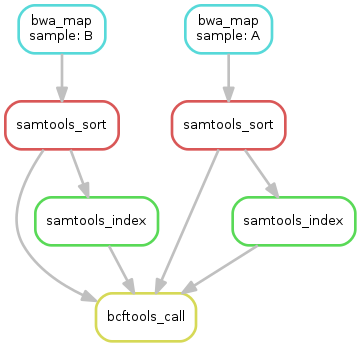
\includegraphics[width=.35\textwidth]{images/dag.png}
    \caption{An example DAG}
    \label{fig:dag}
\end{figure}

\subsection{Generalization of the mapping rule}

In the previous example, one of our input directives was referring to the file \texttt{"data/samples/A.fastq"}. What if we would like to generalise this rule? We can use a wildcard:

\begin{lstlisting}[style=mypython]
rule bwa_map:
    input:
        "data/genome.fa",
        "data/samples/{sample}.fastq"
    output:
        "mapped_reads/{sample}.bam"
    shell:
        "bwa mem {input} | samtools view -Sb - > {output}"
\end{lstlisting}

Both input and output directives have a \texttt{\{sample\}} wildcard. We can notice that the output directive has the same basename of the second input directive. So, to generate the output file, we just need to write:

\begin{lstlisting}[style=mybash]
$ snakemake -np mapped_reads/B.bam
\end{lstlisting}

In this way \texttt{snakemake} will infer that \texttt{B} is a good candidate for the wildcard \texttt{\{sample\}} and then the input file will be \texttt{data/samples/B.fastq} as we desired. Bash expansion can also be used to render this functionality very handy.

\textbf{Note:} Snakemake allows to access wildcards in the shell command via the \texttt{wildcards} object that has an attribute with the value for each wildcard. For example, to use the value of our wildcard in the shell command, we can't use \texttt{\{sample\}}, but we must use \texttt{\{wildcards.sample\}}.

\subsection{Aggregation}

Snakemake provides a helper function for collecting input files that helps us to describe the aggregation in this step. For example, with the following line:

\begin{lstlisting}[style=mypython]
expand("sorted_reads/{sample}.bam", sample=SAMPLES)
\end{lstlisting}

we obtain a list of files where the given pattern \texttt{sorted\_reads/\{sample\}.bam} was formatted with the values in a given list of samples \texttt{SAMPLES}, i.e. \texttt{"sorted\_reads/A.bam"} and \texttt{"sorted\_reads/B.bam"}.

\

We can use multiple wildcards and have their product:

\begin{lstlisting}[style=mypython]
expand("sorted_reads/{sample}.{replicate}.bam", sample=SAMPLES, replicate=[0, 1])
\end{lstlisting}

and then obtain:
\begin{itemize}
    \item \texttt{sorted\_reads/A.0.bam} 
    \item \texttt{sorted\_reads/A.1.bam} 
    \item \texttt{sorted\_reads/B.0.bam} 
    \item \texttt{sorted\_reads/B.1.bam}
\end{itemize}

\subsection{Scripts}

The \texttt{shell} directive is used to specify the rules to generate output files from the input ones. We may also want to make other tasks, for example generating statistics. This can be done with proper scripts. Since the script logic should be separated from the workflow logic, \texttt{snakemake} provides the \texttt{script} directive through which we can invoke a proper Python or R script. In that script, all the properties of the rule like input, output, wildcards, etc. are available as attributes of a global \texttt{snakemake} object.

Let's see a simple example. The following is our simple rule:

\begin{lstlisting}[style=mypython]
rule plot_quals:
    input:
        "calls/all.vcf"
    output:
        "plots/quals.svg"
    script:
        "scripts/plot-quals.py"
\end{lstlisting}

The content of the script \texttt{plot-quals.py} is reported in the following listing:

\begin{lstlisting}[style=mypython]
import matplotlib
matplotlib.use("Agg")
import matplotlib.pyplot as plt
from pysam import VariantFile

quals = [record.qual for record in VariantFile(snakemake.input[0])]
plt.hist(quals)

plt.savefig(snakemake.output[0])
\end{lstlisting}

\subsection{Best practices}

It is best practice to have a rule named \texttt{all} \textbf{at the top} of the workflow which has all typically desired target files as input files. This rule is placed on top because \texttt{snakemake} considers the first rule of the workflow as default target. Apart from this, the appearance of rules in the \texttt{snakefile} is arbitrary and does not influence the DAG of jobs.

\section{Main Commands}

\begin{itemize}

    \item Ask the generation of a given output file (\texttt{snakemake} will determine how to do it):

\begin{lstlisting}[style=mybash]
$ snakemake content_of_output_directive
\end{lstlisting}

    \item Generate a visual representation of the DAG of dependencies:
    \begin{lstlisting}[style=mybash]
$ snakemake --dag | dot -Tsvg > dat.svg
    \end{lstlisting}

    \item See what rules and commands would be executed:
    
    \begin{lstlisting}[style=mybash]
$ snakemake --dryrun --printshellcmds
    \end{lstlisting}

\end{itemize}

\section{References}
\begin{itemize}
\item[\faExternalLink] \href{https://snakemake.readthedocs.io/}{Snakemake documentation}
\item[\faExternalLink] \href{https://www.youtube.com/watch?v=9HxTURMP_Uc}{Snakemake - Reproducible and Scalable Bioinformatic Workflows}
\item[\faExternalLink] \href{https://www.chpc.utah.edu/presentations/snakemake/workflows_with_snakemake.pdf}{The Snakemake Workflow Manager}
\end{itemize}

\end{document}